\section{Communication with Heicub}
\label{sec::34_co}


With YARP, it is possible to directly interface the robot's motors, the cameras, and the force torque sensors. Moreover, it enables the user to run multiple programs in parallel, which can then communicate with each other. A part of the pattern generation library therefore implements rate threads with YARP, which are periodically being called and perform different tasks, such as the generation of dynamically balanced motion, and the decision taking via a neural network.  


which relies on YARP \cite{metta2006yarp} to do the communication between the executing computer, and the robot, see figure \ref{fig::3_yarp}. 





the communication within the control loop is done via YARP \cite{metta2006yarp}, which works for the real robot, as well as for the simulated model in Gazebo \cite{koenig2004design} (figure \ref{fig::3_yarp}). 



It enables the user to implement control loops, like the one that got already shown in figure \ref{fig::31_pg}.

The next section - Code Structure and Usage, will therefore be mainly committed to 




\begin{figure}[h!]
	\centering
	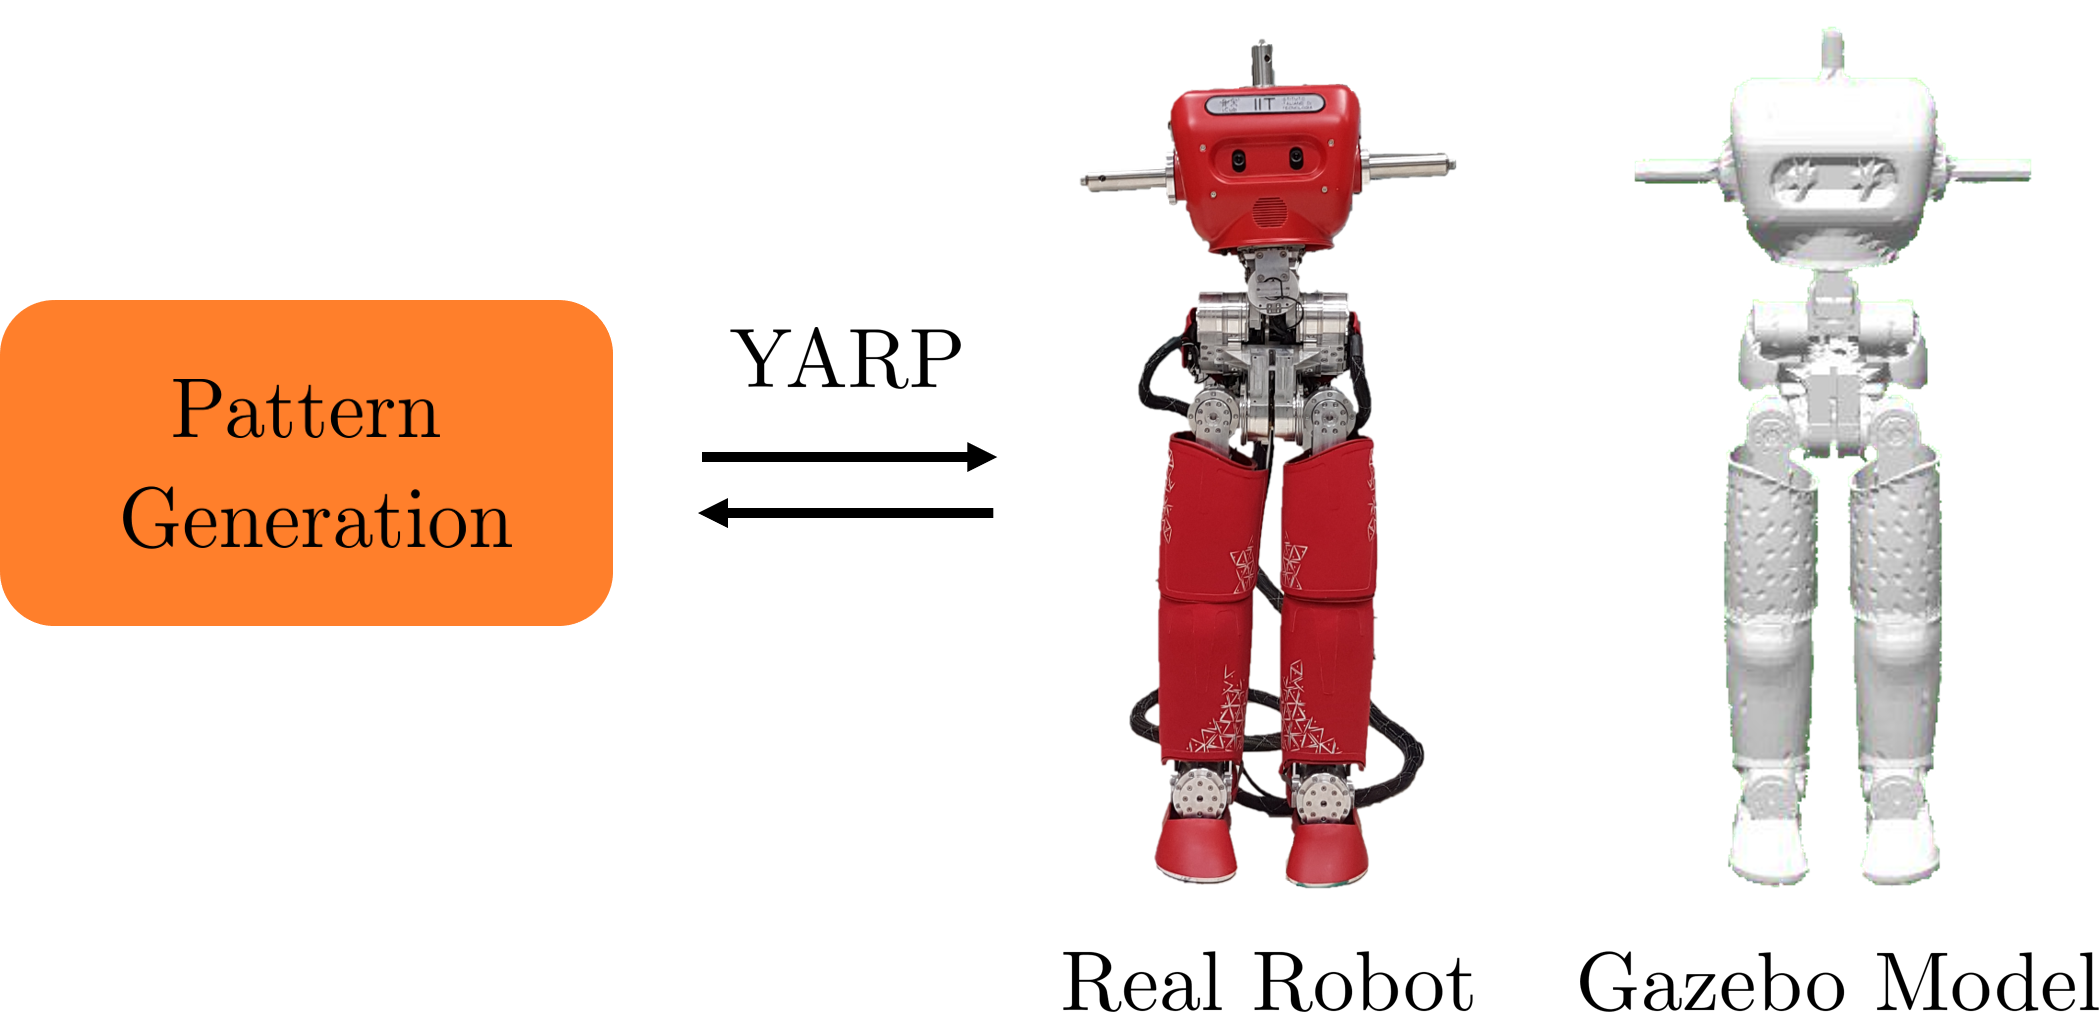
\includegraphics[scale=.25]{chapters/04_methods/img/yarp.png}
	\caption{The pattern generation communicates to the real, or the simulated model, via YARP to access the joint motors and encoders, as well as the cameras, and the force torque sensors.}
	\label{fig::3_yarp}
\end{figure}
A part of the f 
